\documentclass[aps,prd,preprint,superscriptaddress,tightenlines,nofootinbib,floatfix]{revtex4}

%%%%%%%%%%%%%% Use for PRL
%\documentclass[aps,prl,twocolumn,superscriptaddress,showpacs]{revtex4}

%%%%%%%%%%%%%% Use for PRD submission
%\documentclass[aps,prd,preprint,nopreprintnumbers,nofootinbib,showpacs]{revtex4}
%%%%%%%%%%%%%% Use for PRD formatting tables and figures in 2 column
%\documentclass[aps,prd,twocolumn,nofootinbib,showpacs]{revtex4}

\usepackage{graphicx}% Include figure files
\usepackage{dcolumn}% Align table columns on decimal point
\usepackage{bm}% bold math
\usepackage{multirow}% multirow table entries
\usepackage{amsmath}

\begin{document}

%-Definitions-----------------------------------------------------------

\newcommand{\etal}{{\it et al.}}
\newcommand{\ee}{$e^+e^-$}
\newcommand{\mm}{$\mu^+\mu^-$}

\newcommand{\subs}[1]{{\mbox{\scriptsize #1}}}
\newcommand{\re}{\mathrm{Re\:}}
\newcommand{\gee}{$\Gamma_{ee}$}
\newcommand{\ups}{$\Upsilon$}
\newcommand{\uone}{$\Upsilon(1S)$}
\newcommand{\utwo}{$\Upsilon(2S)$}
\newcommand{\uthree}{$\Upsilon(3S)$}
\newcommand{\mpprec}{$m_\subs{$\pi\pi$-rec}$}
\newcommand{\bbar}{$b\bar{b}$}
\newcommand{\inv}{$^{-1}$}
\newcommand{\twotoone}{$\Upsilon(2S) \to \pi^+\pi^- \Upsilon(1S)$}
\newcommand{\pip}{$\pi^+\pi^-$}
\newcommand{\tautau}{$\tau^+\tau^-$}
\newcommand{\dxy}{$d_{XY}$}
\newcommand{\dz}{$d_Z$}

%-----------------------------------------------------------------------
%-----------------------------------------------------------------------
%-----------------------------------------------------------------------

%\preprint line(s) will be ignored for PRL/PRD
%\preprint{CLEO Draft YY-NNA} % For paper draft CBX YY-NN -> Draft YY-NNA
%\preprint{CLEO CONF YY-NN}   % For conference papers
%\preprint{ICHEP ABSnnn}      % For conference papers
%% \preprint{CLNS 05/XXXX; CLEO 05-XX}       % for CLNS notes
%% \preprint{EPS-XXX}         % for CLNS notes
\preprint{CLEO CBX 05-41}

\title{Di-electron Widths of the Upsilon(1S,2S,3S) Resonances}

%% \thanks{Archived as hep-ex/XXXXXXX; 
%% submitted to {\it Phys. Rev. Q}}

%-------- INSERT HERE ------------
% Your author list goes here  REMOVE EVERYTHING to END INSERT and
% replace with your authorlist (ask cleoac).

\author{J.~Pivarski}
\author{J.~R.~Patterson}
\author{K.~Berkelman}
\affiliation{F.~R.~Newman Laboratory for Elementary-Particle Physics, Ithaca, New York 14850-8001}
%\author{(CLEO Collaboration)} %FOR PRD_SPECIAL_CHANGEME
\collaboration{CLEO Collaboration} %FOR PRL,CLNS
\noaffiliation

%\author{John Doe}
%\affiliation{Physics Department, Cornell University
%Ithaca, New York 14853}
%\author{(CLEO Collaboration)}     %FOR PRD_SPECIAL_CHANGEME
%\collaboration{CLEO Collaboration} %FOR PRL and CLNS (superscriptaddress)
%\noaffiliation

%-------- END INSERT ------------

%please hard code the date when you have a final draft and submit to CLEOAC
\date{July 11, 2005}

%---------------------------------------------------------------------
%
%\abstract
%
%---------------------------------------------------------------------

\begin{abstract} 
We have determined the di-electron widths (\gee) of the \uone, \utwo,
and \uthree\ to be
1.339 $\pm$ 0.009 {\it (stat)} $\pm$ 0.020 {\it (syst)} keV,
0.618 $\pm$ 0.010 $\pm$ 0.009 keV, and
0.425 $\pm$ 0.009 $\pm$ 0.006 keV,
respectively.  To measure these widths to their 2\% precisions, the
Cornell Electron Storage Ring scanned the production cross-section
lineshapes of the three resonances in \ee\ collisions, providing the
CLEO detector with a total of 0.61 fb\inv\ of lineshape data and 0.76
fb\inv\ below resonance for background subtraction.  These
measurements are a precise check on lattice QCD calculations for an
observable related to $f_B$.
\end{abstract}
\pacs{13.20.He}  %% what's this?
\maketitle

%---------------------------------------------------------------------
%
\section{Introduction}
%
%---------------------------------------------------------------------

\begin{figure}[t]
  \begin{center}
    \includegraphics[width=0.9\linewidth]{../plots/proceedings_diagrams}
  \end{center}
  \caption{\label{fig:diagrams} Feynman diagrams for (a) the process
  whose probability is measured by \gee, (b) the process for $f_B$.}
\end{figure}

The di-electron width, \gee, of \uone, \utwo, and \uthree\ measures
the coupling of the \bbar\ resonance to a two-electron state.
In the absence of other \ups\ decays, \gee\ would be the inverse
lifetime of the \ups\ and the full-width at half-maximum of the \ups's
rest mass distribution.  Since \ups\ does decay to other final states,
$\Gamma_{ee} = \mathcal{B}_{ee} \Gamma$, and represents about 1 keV of
the \ups's 50 keV full width.  Given $\mathcal{B}_{ee}$, \gee\ is used
to determine $\Gamma$.

The $\Upsilon \to e^+e^-$ process consists of two steps: first the two
$b$ quarks must find each other and annihilate, then \ee\ are produced
electromagnetically through a virtual photon (see Figure
\ref{fig:diagrams}-a).  This second step is well-understood QED, and
can be used as a probe of the QCD involve in the first.  For instance,
the \bbar\ spatial wavefunction, evaluated at the origin, can be
calculated from
\begin{equation}
  |\psi(0,0,0)|^2 = \left(\frac{3 {M_\Upsilon}^2}{16 \pi
   {\alpha_\subs{QED}}^2} \right) \Gamma_{ee} \label{eqn:psi000}
\end{equation}
because the two $b$ quarks must fluctuate to the same point in space
before annihilation \cite{ps}.  This gives us some idea of the width
of the wavefunction in space, and therefore the strength of the force
that binds the two quarks.

Most importantly, \gee\ can test the newly ``unquenched'' lattice QCD
calculations \cite{davies} because it can be calculated to high
accuracy (2--5\%).  This anticipated theoretical accuracy is better
than the current experimental precision of \gee\ (for the \utwo\ and
\uthree\ at least), so a new set of high-precision measurements would
test the predictive power of the unquenched techniques.  Also, notice
the similarity of the process measured by \gee\ and that of $f_B$
(Figure \ref{fig:diagrams}): the QCD part differs only in the mass of
one quark in a central force problem.  Verification of the lattice
\gee\ calculation would lend credence to a lattice $f_B$ calculation.

%---------------------------------------------------------------------
%
\section{Measurement Technique, Datasets, and Detector}
%
%---------------------------------------------------------------------

Perhaps surprisingly, \gee\ is not measured by observing $\Upsilon \to
e^+e^-$, but by observing $e^+e^- \to \Upsilon$.  This is because the
50 keV full width is too narrow to be measured directly, and $\Upsilon
\to e^+e^-$ can only be used to get $\mathcal{B}_{ee}$.  The
production process, $e^+e^- \to \Upsilon$, is related to the decay by
time-reversal symmetry, provided we integrate over initial-state \ee\
energies.
\begin{equation}
  \Gamma_{ee} = \frac{{M_\Upsilon}^2}{6\pi^2} \int \sigma(e^+e^- \to
  \Upsilon) \, dE, \label{eqn:geesig}
\end{equation}
where $\sigma$ is the production cross-section \cite{pdg} \cite{ps}.

We measure the \ups\ production cross-section at the Cornell Electron
Storage Ring (CESR) as a function of incident beam energy (a tunable
parameter), and call this distribution the lineshape.  (It is a
spectral line in analogy with the short-lived excited states of
hydrogen.)  The area under this lineshape, if it were a pure
Breit-Wigner resonance, is the integral needed by Equation
\ref{eqn:geesig}.  The energy spread of the \ee\ is 0.04\% of the beam energy, or about 4
MeV near the \ups\ mass, and this convolves the Breit-Wigner with a
Gaussian that obscures its natural width but preserves its area
exactly.  Another complication is that high-energy \ee\ beams can
radiate a photon before colliding, reducing their energy to the \ups\
mass-energy, and then produce an \ups\ state.  This raises the cross-section
on the high-energy side of the resonance peak.  This (divergent)
high-energy tail should not be included in the integral, so \gee\ is
measured by fitting the observed lineshape to a three-way convolution
of Breit-Wigner, Gaussian, and initial-state radiation tail
(calculated by Kuraev and Fadin \cite{kf}) \cite{kb} with the Breit-Wigner area
as a floating parameter (see Figure \ref{fig:cartoon}).

\begin{figure}[t]
  \begin{center}
    \includegraphics[width=0.6\linewidth]{../plots/proceedings_cartoon}
  \end{center}
  \caption{\label{fig:cartoon} A cartoon of the \gee\ measurement: we
    observe the shape of the Breit-Wigner, Gaussian, ISR tail
    convolution in cross-section versus beam energy and fit for the
    area of the Breit-Wigner.}
\end{figure}

CESR devoted 0.10 fb\inv, 0.06 fb\inv, and 0.10 fb\inv\ to scans of
the \uone, \utwo, and \uthree\ lineshapes between November 2001 and
August 2002.  Each resonance was scanned once a week, and each weekly
scan covered the entire resonance to be able to act as an independent
measurement of \gee.  This is because we were wanted to minimize
sensitivity to weekly shifts in beam energy calibration: the beam
energy is measured with an NMR probe in a test magnet in series with
the ring magnets, and it may be displaced by machine studies.

In addition to the dedicated scan data, we included general-purpose
off-resonance and on-resonance data as points in the lineshape.
Off-resonance data were collected about 20 MeV below each resonance
(0.18 fb\inv, 0.44 fb\inv, and 0.16 fb\inv), which is far enough from
the resonance that they are insensitive to weekly shifts in beam
energy.  The off-resonance data have been combined into three
cross-section measurements, one for each resonance.  On-resonance data
are sensitive to beam energy fluctuations, so only data within 48
hours of a scan are used (0.17 fb\inv, 0.03 fb\inv, 0.15 fb\inv).

The \ups\ cross-section was measured at each energy point by CLEO, a
nearly $4\pi$ general-purpose detector built around the CESR collision
point \cite{cleo}.  This analysis only made use of the central drift chamber and
inner silicon vertex detector for charged particle tracking (in a
solenoidal magnetic field) and the CsI crystal calorimeter for
measuring the energies and trajectories of neutral particles.  The
CLEO trigger accepts events that have a minimum number of trigger
tracks (AXIAL if observed in the first 16 drift chamber layers, STEREO
if extended into the remaining 31) and calorimeter clusters (CBLO if a
calorimeter tile measures more than 150 MeV, CBMD if 750 MeV, and CBHI
if 1.5 GeV).  Our analysis trigger accepts events with at least
\begin{multline}
  \mbox{(3 AXIAL and 1 CBLO) or} \\
  \mbox{(2 STEREO and (2 CBLO or 1 CBMD)) or} \\
  \mbox{(1 AXIAL and 1 CBMD).} \label{eqn:trig}
\end{multline}
We will also make use of a two-track trigger (2 AXIAL tracks,
prescaled by a factor of 20) and a Gamgam trigger (2 CBHI on opposite
sides of the calorimeter barrel) for $e^+e^- \to \gamma\gamma$.

CLEO data were taken in one-hour runs that correspond to fills of the
electron storage ring.  About 2\% of the relevant runs were excluded
because of trigger and event selection inefficiencies peculiar to
these runs.

The detector is simulated with a Monte Carlo based on GEANT \cite{geant}, with
\ups\ events generated by EvtGen \cite{evtgen}, which calls JetSet 7.4 \cite{jetset} for
hadronization.

%---------------------------------------------------------------------
%
\section{Cross-section Measurement}
%
%---------------------------------------------------------------------

The central objective of this analysis is to produce a plot of \ups\
cross-section versus energy, which can be fitted for \gee.  We will
first establish a set of selection criteria (``cuts'') which define a
sample of \ups\ decays, and estimate the number of false positives in
this sample.  Having subtracted these backgrounds from our \ups\
count, we will then consider the inverse problem: how many \ups\
events were left out.  This can be determined directly for \uone\
events, as the decay \twotoone\ provides two charged tracks (\pip)
which can be used to identify the event with little ambiguity.  From
this second, unbiased sample, we count the fraction of \uone\ events
which satisfy our cuts, thus measuring the cuts' efficiency for \uone\
decays without assuming a set of decay modes.  The more energetic
states, \utwo\ and \uthree, can decay the same ways as the \uone, but
can additionally cascade to lower-energy \bbar\ bound states (such as
\uone\ or $\chi_b(1P)$) before the $b$ quarks annihilate.  This adds a
correction to the \utwo\ and \uthree\ efficiencies, but it can be
simulated with Monte Carlo.

Then we will have a true number of $e^+e^- \to \Upsilon$ events, but
this is a function of the luminosity of the \ee\ beams and the length
of time we collected data.  We therefore divide by the time-integrated
luminosity to obtain a cross-section.  %% This factor is determined by
%% counting a subset of ``Gamgam'' ($e^+e^- \to \gamma\gamma$) events and
%% normalizing them to a Monte Carlo prediction of their rate for a given
%% luminosity.  The $e^+e^- \to \Upsilon$ cross-section in the same
%% data-taking period is
%% \begin{equation}
%%   \sigma_{e^+e^- \to \Upsilon} \mbox{ (nb)} = \frac{\#(e^+e^- \to
%%   \Upsilon)}{\#(e^+e^- \to \gamma\gamma)} \, \times \, \frac{\mbox{predicted }
%%   \#(e^+e^- \to \gamma\gamma)}{\mbox{integrated luminosity (nb\inv)}}
%% \end{equation}
We determine the integrated luminosity of a given run by counting a
subset of ``Gamgam'' ($e^+e^- \to \gamma\gamma$) events in that run
and normalizing this count to the known integrated luminosity of the
off-resonance data.
The Gamgam event type is strictly proportional to integrated luminosity because
it has negligible background from
\ups\ decays, as $\Upsilon$ and $\gamma\gamma$ have incompatible
C-parity.

%---------------------------------------------------------------------
%
\subsection{Selection Criteria and Backgrounds} \label{sec:back}
%
%---------------------------------------------------------------------

To suppress large continuum backgrounds such as Bhabhas ($e^+e^- \to
e^+e^-$), we select only hadronic events, that is, all \ups\ decays
except $\Upsilon \to e^+e^-$, $\Upsilon \to \mu^+\mu^-$, and $\Upsilon
\to \tau^+\tau^-$.  The \ups\ efficiency then consists of two factors:
the efficiency of hadronic decays and $1/(1 - 3
\mathcal{B}_{\mu\mu})$, which corrects for the missing leptonic modes
by assuming each to have the same branching fraction (Lepton
Universality) \cite{pdg}.  We will show that the hadronic efficiency is very
high: 96--98\% of hadronic \ups\ decays pass all cuts.

To discriminate against \ee\ and \mm\ final states, which usually
generate two beam-energy tracks, we require the largest track momentum
($\times c$) to be less than 80\% of the beam energy.  This cut
eliminates over 99\% of \ee\ and \mm.  The remaining Bhabha
background, along with continuum hadrons ($e^+e^- \to q\bar{q}$) which
are indistinguishable from hadronic \ups\ decays, contribute to a flat
mesa below the \ups\ resonance lineshape (see Figure
\ref{fig:awesome}).  These backgrounds are effectively subtracted by
adding a $1/s$ term ($s$ = beam energy squared) to the lineshape fit
function and including the off-resonance cross-section measurement as
a point in the fit.

\begin{figure}[p]
  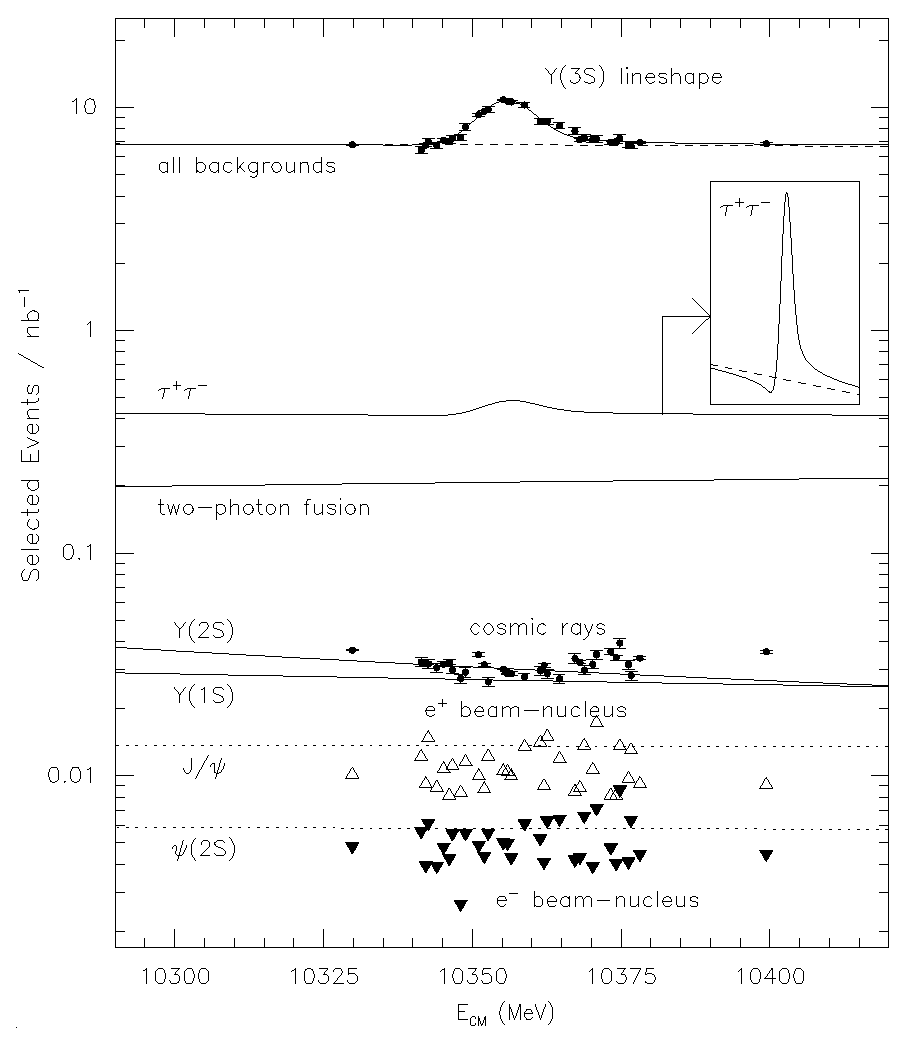
\includegraphics[width=\linewidth]{../plots/awesome}

  \caption{\label{fig:awesome} All \uthree\ backgrounds (\uone\ and
  \utwo\ backgrounds are smaller).  \vspace{0.2 cm} \\
  Lines, top to bottom: fitted lineshape, all backgrounds (dashed),
  continuum and resonance \tautau, with interference (see inset:
  dashed is continuum without resonance); two-photon fusion, which
  rises as $\log s$; \utwo\ and \uone\ high-energy tails, which
  descend as $1/(E-M_\Upsilon)$; $J/\psi$ and $\psi(2S)$ tails
  (dotted), which are not corrected for (they contribute to
  ``two-photon''). \vspace{0.2 cm} \\ Points, top to bottom: observed
  lineshape, cosmic rays (with statistical uncertainties),
  positron-induced beam-gas (open triangles), and electron-induced
  beam-gas (filled triangles).}
\end{figure}

Not all backgrounds, however, depend on beam energy as $1/s$.
Two-photon fusion, in which the incident \ee\ do not collide but emit
virtual photons which do, depends on beam energy as $\log s$.  Most of
these events have low visible energy, the sum of all charged particle
energies (measured by their track momenta, assuming pion masses) and
neutral particle energies (measured by calorimeter showers that cannot
be matched to any charged tracks).  Two-photon fusion events usually
generate little visible energy in the detector because much of the
initial state energy is carried down the beampipe by one or both of
the incident beams that failed to collide.  We only accept events in
which more than 40\% of the center-of-mass energy is visible.  This
cut eliminates most of the two-photon events, which peak below 20\%
(see Figure \ref{fig:visen}).  We gauge the fraction of two-photon
events that survive this cut by fitting the three off-resonance data
points for deviations from $1/s$: correcting for high-energy tails
from \uone\ and \utwo, the fraction of two-photon events at 9 GeV
returned by the fit is (8.0 $\pm$ 0.5)\% (see Figure
\ref{fig:backfit}).  This 8\% may include other non-$1/s$
contributions (such as $J/\psi$ tails, variation in continuum cut
efficiency, or variation in $R$), but we only need to know the shape
of the background for the lineshape fits, not its exact composition.

\begin{figure}[p]
  \begin{center}
    \includegraphics[width=0.9\linewidth]{../plots/proceedings_visen}
  \end{center}
  \caption{\label{fig:visen} Visible energy of off-resonance data
    (solid histogram), showing a large peak of two-photon background
    below 20\% of the center-of-mass energy.  The dotted line
    indicates the cut threshold and the dashed histogram shows \ups\
    events on top of the background (from on-resonance data).}
\end{figure}

\begin{figure}[p]
  \begin{center}
    \includegraphics[width=0.9\linewidth]{../plots/proceedings_backgrounds}
  \end{center}
  \caption{\label{fig:backfit} The three off-resonance points showing
    \uone\ and \utwo\ tail corrections (corrected points are lower),
    fitted to $1/s + \log s$ (solid line).  The dashed line shows a
    pure $1/s$ fit through \uone\ off-resonance for comparison.}
\end{figure}

This visible energy cut also rejects some \tautau\ events, as these
subsequently decay into final states involving neutrinos.  However,
58\% remain after cuts, and this background is seemingly irreducible
as the final states look like hadronic events: they have two or more
low-momentum tracks without strong geometric correlations.  They are
therefore allowed to contribute to 0.58 $\times$
$\mathcal{B}_{\tau\tau}$ $\approx$ 1\% of the resonance peak.

\begin{figure}[p]
  \includegraphics[width=\linewidth]{../plots/datasets_database_dxydzcuts}
  \caption{\label{fig:cosbg} Two geometric variables used to select
    cosmic rays and beam-gas.  In each case, the histogram is all
    experimental data, and the points are a control (beamless data or
    single-beam data). \vspace{0.2 cm} \\
    (a) \dxy, the distance of closest approach of the
    closest track to the beamline, after other cosmic ray cuts (in log
    $x$ scale: 0.01 is 1 cm).  The distribution above 5 mm (dotted
    line) is well-described by no-beam data. \vspace{0.2 cm} \\
    (b) \dz, the distance of the event vertex from the
    nominal beam spot, as measured along the beamline.  Although
    beam-gas cuts reject events with \dz\ $<$ 7.5 cm (dotted line), the
    beam-gas count may be contaminated by some collision data.}
\end{figure}

Any backgrounds which vary slowly with beam energy and are
proportional to luminosity can be subsumed into the fit parameters
described above.  Cosmic rays, however, will not be proportional to
luminosity as they come from an external source.  We reject most
cosmic rays by requiring that the distance of closest approach of the
closest track to the beamline (\dxy) be less than 5 mm (a very loose
cut: \dxy\ has an RMS of 0.2 mm).  We find the number of cosmic rays
that survive hadronic cuts by applying the cuts to a control dataset
with no beams in CESR (cosmic rays only), normalized by the number of
events satisfying special cosmic ray cuts, for each run.
Figure \ref{fig:awesome} shows the result of this measurement for
\uthree\ data (typically 0.4\% of the continuum), and Figure
\ref{fig:cosbg}-a shows \dxy\ for events that passed all other cosmic
rays cuts, for experimental and control data.

Another two backgrounds which aren't proportional to luminosity are
beam-gas events, in which one beam electron or positron collides with
a gas atom inside the beampipe, and beam-wall, in which a beam
particle collides with the wall of the beampipe.  These are suppressed
by calculating an approximate vertex for each event in Z, along the
beamline (called \dz).  Beam-gas and beam-wall events may occur
anywhere along the beamline, but beam-beam collisions must originate
within a few centimeters of the nominal beam spot.  We cut at 7.5 cm
(also loose: \dz\ has an RMS of 1.5 cm).  To count survivors, we
construct a set of beam-gas cuts and test them in a single-beam
control sample, in analogy to cosmic ray counting above (except that
cosmic rays need to be subtracted from the single-beam sample).
Figure \ref{fig:cosbg}-b shows \dz\ after other beam-gas cuts, for
experimental and control data.  Unlike cosmic rays, which are easily
distinguished from collision data and are well-represented by the
no-beam sample (\ref{fig:cosbg}-a), beam-gas cuts before \dz\ have a
large background from collision data, and the low-precision in the
single-beam sample makes it unclear how many collision events have
large \dz.  As a precaution, we subtract 50\% $\pm$ 50\% of the
estimated beam-gas background from our hadronic event count.
Beam-wall events were found to be much less common than beam-gas, and
are subsumed into this uncertainty.  As the $e^+$ and $e^-$ beams may
have different currents, we count electron-induced beam-gas
independently of positron-induced beam-gas.  (They can be
distinguished by their net Z momentum.)  Beam-gas counts are also
plotted in Figure \ref{fig:awesome}; they typically amount to 0.1\% of
the continuum.

%---------------------------------------------------------------------
%
\subsection{Hadronic Efficiency}
%
%---------------------------------------------------------------------

Now that we know we can subtract non-\ups\ events from our hadronic
event count (or cover the remainder with an uncertainty), we turn to
the issue of hadronic \ups\ decays missing from that count.  These
events may be missing because they are detected but fail our four
cuts, or, more seriously, because they fail to trigger.  For example,
the decay $\Upsilon \to Z^* \to \nu\bar{\nu}$, which is ``hadronic''
by our choice of definition, generates no tracks and no showers.  We
need to put a limit on invisible decays such as this, ideally one that
assumes as little as possible from a theoretical model.  This limit
will dominate the uncertainty in hadronic efficiency.

All \uone\ decays can be seen from \twotoone\ if the two tracks left
by the charged pions are sufficient to satisfy the trigger.  A pion
with more than 150 MeV of transverse momentum will generate an AXIAL
track in the trigger with (99.93 $\pm$ 0.07)\% probability
\cite{inga}.  By requiring both pions to satisfy this criterion and
selecting events from the prescaled two-track trigger, we obtain a
complete and unbiased set of \uone\ decays, though at a cost of a
factor of 20 in sample size.

The \twotoone\ events in this sample are identified by requiring the
recoil mass of the two pions
\begin{equation}
  {m_\subs{$\pi\pi$-rec}}^2 = \left(2 E_\subs{beam} - \sqrt{|\vec{p}_1|^2 + {m_\pi}^2}
  - \sqrt{|\vec{p}_2|^2 + {m_\pi}^2}\right)^2 - |\vec{p}_1 + \vec{p}_2|^2
\end{equation}
to be close to the \uone\ mass.  As can be seen in Figure
\ref{fig:recoil}-a, the \uone\ peak sits on top of a flat background
of random two-track combinations, sometimes from true \twotoone\
decays but often from other event types.  We suppress this
combinatoric background by requiring the pair of tracks to intersect
near the beam spot and to have opposite charges, but ultimately, the
remainder will need to be subtracted by a linear fit.

We first want to learn from this study how many \uone\ events are
``invisible,'' which we will take to mean how many fail to generate
one AXIAL track and one CBLO (150 MeV cluster) in the trigger.  This
is a necessary condition for the analysis trigger, so any event that
fails this simple criterion will fail the exact trigger criteria
described in Equation \ref{eqn:trig}.  We fit the recoil mass peak to
a double Gaussian (Figure \ref{fig:recoil}-a) and use the same mean,
sigmas, and area ratio in a fit to the invisible events (Figure
\ref{fig:recoil}-b).  The ratio of these two is (0.67 $\pm$ 0.62)\%,
so the probability for an \uone\ to be ``visible to the trigger'' is
(99.22 $^{+0.48}_{-0.57}$)\%, after correcting for the fact that
efficiencies must be less than 100\%.

The hadronic efficiency of our cuts can be more precisely determined
because we do not need to use as small a set of \twotoone\ events.
Instead of only considering events from the prescaled two-track
trigger, we can use events from an unprescaled trigger which requires
three AXIAL tracks and one CBLO.  This sample is called low-bias (see
Figure \ref{fig:recoil}-c for a recoil mass plot) because the \uone\
must supply one AXIAL track and one CBLO; e.g., it must be
``visible.''  We apply our hadronic cuts, excluding the two pions, to
this sample and count \#pass/(\#pass $+$ \#fail), first subtracting
scaled sideband events (\mpprec\ $\in$ (9.441, 9.454) $\cup$ (9.472,
9.480) GeV) from signal events (9.454 $<$ \mpprec\ $<$ 9.472 GeV).
Figure \ref{fig:recoil}-d shows the recoil mass of events that failed
the cuts.  This fraction, which includes $\Upsilon(1S) \to e^+e^-$,
$\mu^+\mu^-$, and $\tau^+\tau^-$, is (92.58 $\pm$ 0.13)\%.  Correcting
for leptonic modes, the hadronic cut efficiency is (98.32 $\pm$
0.21)\%.

We repeated this procedure for \twotoone\ Monte Carlo, and obtained a
(98.54 $\pm$ 0.22)\% hadronic cut efficiency, in good agreement with
the data.  We also simulated $e^+e^- \to \Upsilon(1S) \to$ hadronic
modes, in which we found a (98.68 $\pm$ 0.04)\% efficiency: also in
good agreement.  Using the ratio of these Monte Carlo predictions as a
1.0014 $\pm$ 0.0022 correction factor, the $e^+e^- \to \Upsilon(1S)$
hadronic cut efficiency is (98.46 $\pm$ 0.30)\%.

Distributions of the four variables used in our cuts are presented in
Figure \ref{fig:4var}, after subtracting combinatoric backgrounds.
Monte Carlo (\twotoone) is overlaid for comparison.

In general, our analysis trigger requires more than one AXIAL track
and one CBLO.  The trigger efficiency, after our ``visible to
trigger'' condition and hadronic cuts, is 99.87\% in Monte Carlo.  A
comparison of AXIAL, STEREO, CBLO, and CBMD distributions in data and
Monte Carlo indicate that the simulation can be trusted, at the very
least within 100\% of the predicted effect (Figure \ref{fig:mctrig}),
so we will assign it a systematic error of 0.13\%.

The \uone\ hadronic efficiency is (97.57 $^{+0.58}_{-0.66}$)\%, the
product of these three cumulative efficiencies (listed in Table
\ref{tab:fityields}).

\begin{figure}[p]
  \vspace{3 cm}
  \begin{center}
    \Large $\pi^+\pi^-$ recoil mass in GeV
  \end{center}

  \vspace{-1.8 cm}
  \begin{center}
    \includegraphics[width=0.9\linewidth]{../plots/proceedings_fityields2}
  \end{center}
  \caption{\label{fig:recoil} Recoil mass of $\pi^+\pi^-$ in (a) the
    unbiased sample (all \ups\ decays are present), (b) the unbiased
    sample for invisible decays (no AXIAL tracks or no 150 MeV
    clusters), (c) the low-bias sample (\ups\ must be visible), and
    (d) the low-bias sample failing hadronic cuts.  Most of the \uone\
    decays in (d) are lepton pairs.}
\end{figure}

\begin{table}[t]
  \begin{center}
    \begin{tabular}{r l c}
      \hline \hline & Criterion & Efficiency \\ \hline
      1. & Visible to trigger: $\ge$1 AXIAL track and $\ge$ 1 CBLO (150 MeV cluster) & (99.22 $^{+0.48}_{-0.57}$)\% \\ \hline
         & Passed all cuts (assuming visible \uone)                                  & (92.58 $\pm$ 0.13)\% \\
         & Passed all cuts (assuming visible hadronic \uone)                         & (98.32 $\pm$ 0.21)\% \\
      2. & Passed all cuts without boost/track confusion (assuming the above)        & (98.46 $\pm$ 0.30)\% \\ \hline
      3. & Passed trigger (Equation \ref{eqn:trig}, assuming visible and passed cuts)& (99.87 $\pm$ 0.13)\% \\ \hline
         & \uone\ hadronic efficiency (product of 1, 2, and 3)                       & (97.57 $^{+0.58}_{-0.66}$)\% \\ \hline\hline
%%       largest track momentum ($\times c$) $<$ 80\% of beam energy & (94.62 $\pm$ 0.07)\% & \\
%%       visible energy $>$ 40\% center-of-mass energy & (98.76 $\pm$ 0.10)\% & \\
%%       $|d_{XY}|$ $<$ 5 mm & (99.94 $\pm$ 0.02)\% & \\
%%       $|d_{Z}|$ $<$ 7.5 cm  & (99.12 $\pm$ 0.04)\% & \\ \hline \hline
    \end{tabular}
  \end{center}
  \caption{\label{tab:fityields} Summary of cut efficiency
    measurement for \uone.}
\end{table}

\begin{figure}[p]
  \vspace{3 cm}
  \begin{center}
    \includegraphics[width=0.9\linewidth]{../plots/proceedings_cuts3}
  \end{center}
  \caption{\label{fig:4var} The four hadronic cuts, as seen in
    \twotoone\ decays.  Points are data (with combinatoric backgrounds
    subtracted) and histograms are Monte Carlo; dotted lines are cut
    thresholds.  (All cuts are applied except the one presented.)  (a)
    Biggest track momentum $<$ 80\% beam energy (cross-hatched
    histogram is \ee, \mm\ Monte Carlo), (b) visible energy $>$ 40\%
    expected center-of-mass energy, (c) $|d_{XY}|$ $<$ 5 mm, and (d)
    $|d_Z|$ $<$ 7.5 cm.}
\end{figure}

\begin{figure}[p]
  \vspace{3 cm}
  \begin{center}
    \includegraphics[width=0.9\linewidth]{../plots/trigger_lowlevel_1s_2}
  \end{center}
  \caption{\label{fig:mctrig} Trigger variables as seen in hadronic
    data (points) and in Monte Carlo (histogram).  (a) Number of AXIAL
    tracks, (b) STEREO tracks, (c) CBLO (150 MeV clusters), and (d)
    CBMD (750 MeV clusters).  The analysis trigger decision is derived
    from these variables using Equation \ref{eqn:trig} (the lower
    limits are indicated by dotted lines).  Data have been
    continuum-subtracted, cosmic-ray and beam-gas-subtracted, and the
    leptonic modes have been subtracted using Monte Carlo.}
\end{figure}

The \utwo\ and \uthree\ can decay into any final states that the
\uone\ can, but can also cascade into lower \bbar\ resonances.  This
has three implications: the 0.7\% uncertainty in invisible \uone\
decays must be shared by the \utwo\ and \uthree, the efficiency will
need to be corrected for cascade decays, and, in particular, for
cascades in which a lower \ups\ decays into \ee\ or \mm, as these will
be lost to our cuts.

We answer the first two considerations by first correcting the \uone\
efficiency for all cascade decay modes except ``cascades to leptons''
(\ee\ and \mm).  Simulations of $e^+e^- \to \Upsilon(2,3S) \to$
hadrons/taus only predict a (98.45 $\pm$ 0.05)\% efficiency, to be
compared with the (98.68 $\pm$ 0.04)\% \uone\ prediction above.
%% This difference is due to the
%% presence of cascade decays and the higher ratio of $q\bar{q}$ to
%% $ggg$, which are coincidentally the same for \utwo\ and \uthree.
The \uone\ efficiency is therefore corrected by 0.9977 $\pm$ 0.0007,
and this result, (97.35 $^{+0.58}_{-0.66}$)\%, is presented at the top
of Table \ref{tab:fityields23}.

\begin{table}[t]
  \begin{center}
    \begin{tabular}{l c}
      \hline\hline Efficiency of all modes except cascades to leptons (both \utwo\ and \uthree) & (97.35 $^{+0.58}_{-0.66}$)\% \\ \hline
      Efficiency of cascades to leptons from \utwo\ & (0.69 $\pm$ 0.22)\% \\
      Efficiency of cascades to leptons from \uthree\ & (0.38 $\pm$ 0.19)\% \\
      \utwo\ cascade to leptons branching fraction & (1.58 $\pm$ 0.16)\% \\
      \uthree\ cascade to leptons branching fraction & (1.34 $\pm$ 0.13)\% \\ \hline
      \utwo\ hadronic efficiency (aggregate of the two components) \mbox{\hspace{0.8 cm}} & (95.82 $^{+0.58}_{-0.66}$ $\pm$ 0.15)\% \\
      \uthree\ hadronic efficiency (aggregate of the two components) & (96.05 $^{+0.58}_{-0.66}$ $\pm$ 0.13)\% \\ \hline\hline
    \end{tabular}
  \end{center}
  \caption{\label{tab:fityields23} Summary of cut efficiency
    measurement for \utwo\ and \uthree.}
\end{table}

\begin{figure}[t]
  \begin{center}
    \includegraphics[width=0.8\linewidth]{../plots/beautiful_bcasll_2}
  \end{center}
  \caption{\label{fig:beaut} Invariant mass of the two largest tracks
    (divided by $M_\Upsilon$) in \utwo\ and \uthree\ with $X e^+e^-$
    rejected.  Points are continuum-subtracted data, the shaded
    histogram is $\Upsilon(2S,3S) \to \mu^+\mu^-$ (prompt \mm) Monte
    Carlo, and the empty histogram stacked on top of it is
    $\Upsilon(2S,3S) \to X \Upsilon \to X \mu^+\mu^-$ (cascade \mm).
    The Monte Carlo normalizations have been fitted to the data, from
    which the cascade/prompt ratio is determined.}
\end{figure}

The cascade to leptons mode, with two high-energy electrons or muons
in the final state, is usually rejected by our largest track momentum
cut: the efficiency is (0.69 $\pm$ 0.22)\% for \utwo\ and (0.38 $\pm$
0.19)\% for \uthree.  We measured the branching fractions of \utwo\
and \uthree\ to this mode using our on- and off-resonance data.  We
select events with two high-momentum tracks ($>$ 70\% of beam energy),
and reject those with a high-energy shower ($>$ 70\% of beam energy).
After subtracting the appropriately-scaled continuum sample, we are
left with a number of prompt \mm\ ($\Upsilon(2S,3S) \to \mu^+\mu^-$)
and cascade \mm\ ($\Upsilon(2S,3S) \to X \Upsilon \to X \mu^+\mu^-$)
events.  These can be distinguished by the invariant mass of the \mm\
pair, as seen in Figure \ref{fig:beaut}.  We measure the ratio of
cascade/prompt branching fractions by fitting the normalizations of
cascade and prompt Monte Carlo to the data, and obtain the desired
cascades to leptons branching fraction by multiplying by prompt
$\mathcal{B}_{\mu\mu}$ (from \cite{istvan}) $\times$ 2.  The Monte
Carlo does not exactly reproduce the \mm\ invariant mass, which is the
dominant uncertainty ($\lesssim$ 10\% of itself).  The cascades to
leptons branching fractions are (1.58 $\pm$ 0.16)\% for \utwo\ and
(1.34 $\pm$ 0.13)\% for \uthree.

The total hadronic efficiency is an aggregate of the cascade to
leptons part and the non-cascade to leptons part, i.e.,
\begin{eqnarray}
  \epsilon_{MC}(2S) &=& (0.0158) \, 0.69\% + (1 - 0.0158) \, 97.35\% = \mbox{(95.82 $^{+0.58}_{-0.66}$ $\pm$ 0.15)\%} \nonumber \\
  \epsilon_{MC}(3S) &=& (0.0134) \, 0.38\% + (1 - 0.0134) \, 97.35\% = \mbox{(96.05 $^{+0.58}_{-0.66}$ $\pm$ 0.13)\%.} \nonumber
\end{eqnarray}
The first (asymmetric) uncertainty is common to all three resonances,
while the second is from the cascade to leptons measurements, which
dominates the efficiency differences.

%---------------------------------------------------------------------
%
\subsection{Luminosity}
%
%---------------------------------------------------------------------

For each beam energy, we can now count hadronic \ups\ decays, subtract
non-\ups\ backgrounds from this count, and correct it for missing
\ups\ events.  All that remains is to remove the effects of variable
run lengths by converting this number into a cross-section: we need to
measure the integrated luminosity at each energy point.  We have two
concerns: the first is to determine the integrated luminosity of each
measurement up to a single constant, so that observed lineshapes are
undistorted.  We will measure these ``relative luminosities'' by
counting Gamgam events at each energy.  The second concern is to
determine the last constant, the absolute luminosity, turning a number
of Gamgams into nb\inv\ and setting the scale for all three \gee\
measurements.

Gamgam events ($e^+e^- \to \gamma\gamma$) have a distinct signature---
two large, back-to-back showers--- so backgrounds are not an issue
above our level of consideration (0.1\%).  Also, we do not need to
know the efficiency of our Gamgam cuts for a relative luminosity
measurement.  We require there to be no tracks in the drift chamber,
two large ($>$ 70\% of beam energy) showers in the calorimeter which
are back-to-back in $\phi$ (the polar angle around the beamline; we
require $|\sin \phi_1 - \phi_2|$ $<$ 0.04 to avoid the nearly
back-to-back showers from \ee), and back-to-back in $\theta$ (the
azimuthal angle; we require $|\cot\theta_1 + \cot\theta_2|$ $<$ 0.1,
as the calorimeter has a barrel geometry and crystal elements are
equally spaced in $\cot\theta$).  We also restrict ($\theta_1$,
$\theta_2$) to be far from the edge of the calorimeter barrel
($\min(|\cot\theta_1|, |\cot\theta_2|) < 1.18$ and
$\max(|\cot\theta_1|, |\cot\theta_2|) < 1.28$) and far from the center
($\min(|\cot\theta_1|, |\cot\theta_2|) > 0.05$ and
$\max(|\cot\theta_1|, |\cot\theta_2|) > 0.15$).  At the edge, showers
may be clipped, and at the center, the trigger is inefficient.

Since Gamgam events have no tracks, they rely on the back-to-back 1.5
GeV-cluster trigger.  This trigger accepts events with two high-energy
clusters which are moderately back-to-back in $\phi$ (our cut is much
tighter) and on opposite sides of the detector in $\theta$.  Near the
center, both photons may be found on the same side of the detector and
the trigger is inefficient.  We cut this region out.  There are three
other regions where the trigger is inefficient: some calorimeter
trigger tiles were unresponsive for part of \ups\ data-taking.  We
also cut these regions out (for all data).

To \label{pag:lumical} convert these Gamgam counts into nb\inv, the
integrated luminosity of all off-resonance data was measured to be
0.76 fb\inv\ with a fractional accuracy of 1.8\%.  This measurement
used $e^+e^-$, $\gamma\gamma$, and $\mu^+\mu^-$ events, following the
method of~\cite{LUMINS}; event counts were normalized with a Monte
Carlo simulation based on the Babayaga~\cite{babayaga} event
generator.  (The 1.8\% systematic error reflects the agreement of the
$e^+e^-$, $\gamma\gamma$, and $\mu^+\mu^-$ measurements: it is the
root mean square of their values around the mean.)  By comparing the
Gamgam count for off-resonance data with the Gamgam count for any
other measurement, we obtain integrated luminosities which are not
distorted by resonance effects and share a common uncertainty.

%---------------------------------------------------------------------
%
\section{Cross-section and Beam-energy Measurement Stability}
%
%---------------------------------------------------------------------

%---------------------------------------------------------------------
%
\subsection{Cross-section Measurement Stability} \label{sec:csstab}
%
%---------------------------------------------------------------------

We primarily use the drift chamber to count hadronic events and the
calorimeter to count Gamgams, so the cross-section relies on these two
detectors being synchronized.  If one fails while the other continues to count,
the measured cross-section will be too low or too high.

The calorimeter can fail to count a Gamgam event if one of the two
photons enters a tile which isn't read out by the trigger.  This is
why we rejected these regions with our Gamgam cuts, to stabilize the
count by making these regions always inefficient.  We measure the
Gamgam trigger efficiency by selecting Bhabhas with the drift chamber
and asking how often the Gamgam trigger is satisfied by the two
energetic electrons.  For good runs, the Gamgam trigger is 99.7\%
efficient after cuts, with a $\sim$0.2\% statistical precision in each.

The drift chamber can fail if it looses high voltage and therefore
sensitivity to all charged particles.  We checked for drift chamber
insensitivity by selecting Bhabhas with the calorimeter ($0.04 < |\sin
\phi_1 - \phi_2| < 0.25$) and asking how often the drift chamber
trigger failed to see one AXIAL track.  In good runs, at most 0.3\% of
Bhabhas have no tracks (Gamgam might be a background).

A way to check the stability of the luminosity measurement is to
compare Gamgam counts with Bhabha counts off-resonance, where the
\ups\ background is minimal.  The Gamgam/Bhabha ratio is 0.0793 $\pm$
0.0002, 0.0792 $\pm$ 0.0001, and 0.0793 $\pm$ 0.0002 for the three
measurements, all in statistical agreement and very precise (0.2\%).

To put an upper limit on cross-section instability, we consider the
consistency of all off-resonance runs at the same energy with a
common cross-section measurement.  The negative log likelihood of
this agreement is
\begin{equation}
  L(\delta_x) = \sum_{i=1}^{526} -\ln \left(\frac{1}{\sqrt{2\pi
  ({\delta_{\sigma_i}}^2 + {\delta_x}^2)}} \exp\left(-\frac{(\sigma_i
  - \langle\sigma\rangle)^2}{2 ({\delta_{\sigma_i}}^2 + {\delta_x}^2)}
  \right)\right)
\end{equation}
where $\sigma_i$ $\pm$ $\delta_{\sigma_i}$ are the individual
cross-section measurements, $\langle\sigma\rangle$ is their mean
(different below each resonance), and $\delta_x$ is a hypothetical
fluctuation in cross-section beyond the statistical error.  To raise
$L(\delta_x)$ above $L(0)$ by 0.5, a $\delta_x$ of 0.03 nb is needed.
This is smaller than the typical statistical error of 0.2 nb, and is
derived from a larger dataset than the lineshape scans.  An $S$-factor
in analogy to the PDG's can't be used here, as $S(0)$ $<$ 1.

Fitting simulations with this small error indicate that it can change
the value of \gee\ by only 0.1\%.

%---------------------------------------------------------------------
%
\subsection{Beam-energy Measurement Stability} \label{sec:energy}
%
%---------------------------------------------------------------------

We minimized our sensitivity to fluctuations in the beam energy
measurement by collecting data in small, independent scans, and by
alternating measurements above and below the \ups\ mass.  To determine
the stability of this measurement, most weekly scans included two
cross-section measurements at the same energy, usually near the
beginning and end of the scan and at a point where the lineshape has a
high derivative.  If the beam energy calibration does not fluctuate
between the two measurements, the hadronic cross-sections should be
statistically consistent.  If it fluctuates by a large amount, we
would see a different hadronic cross-section, and can divide this
difference by the derivative of the lineshape to measure the shift in
beam energy calibration.  If the beam energy fluctuates rapidly, many
times during a single cross-section measurement, this contributes to
the natural beam energy spread and is not relevant.  Note that the
calibration shifts under consideration here must take place during a
weekly scan, not between them, as only these can distort the
lineshape.

We converted thirty pairs of repeated measurements into beam energy
calibration shifts, and plotted them in Figure \ref{fig:miscal} as a
function of time between the end of the early and the beginning of the
late measurement.  As there is no evidence of any calibration shift,
we construct an upper limit the same way we did for cross-section
stability:
\begin{equation}
  L(\delta_E) = \sum_{i=1}^{30} -\ln \left(\frac{1}
  {\sqrt{2\pi ({\delta_{s_i}}^2 + {\delta_E}^2)}} \exp\left(
  -s_i^2 / 2 / ({\delta_{s_i}}^2 + {\delta_E}^2) \right) \right)
\end{equation}
where $s_i$ $\pm$ $\delta_{s_i}$ are the calibration shift
measurements plotted in Figure \ref{fig:miscal}, and $\delta_E$ is an
assumed uncertainty in beam energy.  To raise $L(\delta_E)$ above
$L(0)$ by 0.5, a $\delta_E$ of 0.05 MeV is needed.  An $S$-factor in
analogy to the PDG's would set $\delta_E$ at 0.07 MeV.

\begin{figure}[t]
  \begin{center}
    \includegraphics[width=0.9\linewidth]{../plots/proceedings_miscal}
  \end{center}
  \caption{\label{fig:miscal} Beam energy calibration shifts, as
    determined from thirty pairs of repeated cross-section
    measurements (plotted versus time).}
\end{figure}

Fitting simulations with a $\delta_E$ of 0.05 MeV or 0.07 MeV indicate
that it can change the value of \gee\ by 0.2\%.

%---------------------------------------------------------------------
%
\section{Fitting}
%
%---------------------------------------------------------------------

For each resonance lineshape fit, the background level $\sigma_b$ is
allowed to float: the $1/s + \log s$ background shape is only
extrapolated 50 MeV or so within an \ups\ lineshape.  The Breit-Wigner
area (\gee) also floats, as does the beam energy spread $\Delta E$.
Also, the peak position of each weekly scan (12 for \uone, 6 for \utwo, and
7 for \uthree) floats in the fit.  By this, we mean that data
from one week can slide up and down in beam energy independently of
data from another week, while the theoretical lineshape is fixed at
the known \ups\ mass.

The peak fit function is a convolution of a Breit-Wigner, a Gaussian,
and an initial-state radiation tail, with an interference term between
the Breit-Wigner and the continuum background.  The \ups\ has a 10\%
branching fraction to $q\bar{q}$, and $e^+e^- \to q\bar{q}$ is the
primary component of the continuum.  In principle, the observed
cross-section is not the sum of these two, but is proportional to the
squared sum of their amplitudes:
\begin{eqnarray}
  \sigma(e^+e^- \to X \to q\bar{q}) &\propto& |\mathcal{M}(e^+e^- \to q\bar{q}) + \mathcal{M}(e^+e^- \to \Upsilon \to q\bar{q})|^2 \\
  &\propto& |\mathcal{M}(e^+e^- \to q\bar{q})|^2 + |\mathcal{M}(e^+e^- \to \Upsilon \to q\bar{q})|^2 + \nonumber \\
  & & \mbox{\hspace{1.5 cm}} 2 \, \mathrm{Re\:} \mathcal{M}(e^+e^- \to q\bar{q})^* \mathcal{M}(e^+e^- \to \Upsilon \to q\bar{q}) \mbox{.}
\end{eqnarray}
The last term is the interference term, and it distorts the \ups\
lineshape by causing a deficit of events below the \ups\ mass and an
excess above it.  The data, however, are not statistically sensitive
to this effect.  (The interference term, at its maximum, is about a
factor of 70 smaller than the peak at its maximum.)

As previously mentioned, 58\% of $\Upsilon \to \tau^+\tau^-$ survive
hadronic cuts, so these are added as a contribution to the fit
function.  These events have the same lineshape as the hadronic
decays, except for an interference term which is larger by a factor of
10 relative to its peak (see the inset in Figure \ref{fig:awesome}).

The background has the $1/s + \log s$ shape described in Section
\ref{sec:back}, plus tails from \uone\ and \utwo.

The \uone, \utwo, and \uthree\ lineshape fits are presented in Figure
\ref{fig:fits} with pull distributions in Figures \ref{fig:pull1},
\ref{fig:pull2}, and \ref{fig:pull3}.  Fit results are presented in
Table \ref{tab:fits}: the statistical uncertainties of 0.7\%, 1.6\%,
and 2.2\% are dominated by Gamgam counting.  The \uone\ reduced
$\chi^2$ is moderately high (1.2, with a 4\% C.L.), but a combined
$\chi^2$ of the three fits is 442.6/426 = 1.04, with a 28\% confidence
level.

Systematic uncertainties from varying each fixed parameter are listed
in Table \ref{tab:lineshape}, all of which are very small.  The
largest, theoretical error in the calculation of the high-energy tail,
is shared by all three resonances.

\begin{table}
  \begin{center}
%%    \renewcommand{\arraystretch}{1.25}
    \begin{tabular}{l c c c}
      \hline\hline
      & \uone & \utwo & \uthree \\\hline
      & & & \vspace{-0.4 cm} \\
      $\chi^2/$\#degrees of freedom & $\displaystyle \frac{229.8}{210-15}$ = 1.18 & $\displaystyle \frac{57.6}{75-9}$ = 0.87 & $\displaystyle \frac{155.2}{175-10}$ = 0.94 \\
      Confidence level & 4\% & 76\% & 70\% \\
      $\int \sigma(e^+e^- \to \Upsilon \to \mbox{hadrons}) \, dE$ (in MeV nb) & 318.9 $\pm$ 2.1 & 133.2 $\pm$ 2.1 & 84.9 $\pm$ 1.9 \\
      $\int \sigma(e^+e^- \to \Upsilon) \, dE$ (in MeV nb) & 345.0 $\pm$ 2.4 & 141.9 $\pm$ 2.3 & 91.5 $\pm$ 2.0 \\
      Statistical uncertainty & 0.7\% & 1.6\% & 2.2\% \\ \hline\hline
    \end{tabular}
%%    \renewcommand{\arraystretch}{1.}
  \end{center}
  \caption{\label{tab:fits} Fit results.}
\end{table}

\begin{table}
  \begin{center}
    \begin{tabular}{l c c c}
      \hline\hline
      & \mbox{\hspace{0.5 cm}} \uone\ \mbox{\hspace{0.5 cm}} & \mbox{\hspace{0.5 cm}} \utwo\ \mbox{\hspace{0.5 cm}} & \mbox{\hspace{0.5 cm}} \uthree\ \mbox{\hspace{0.5 cm}} \\\hline
      From uncertainty in the full-width $\Gamma$                                 & 0.005\% & 0.02\%  & 0.03\% \\
      Interference term for $q\bar{q}$ (depends on $\mathcal{B}_{\mu\mu}$, $R$)   & 0.02\%  & 0.02\%  & 0.002\% \\
      Interference term for $\tau^+\tau^-$ (depends on $\mathcal{B}_{\tau\tau}$)  & 0.08\%  & 0.07\%  & 0.05\% \\
      Two-photon fraction                               	   		  & 0.002\% & 0.002\% & 0.001\% \\
      Initial-state radiation tail (0.1\% theory error) 	   		  & 0.05\%  & 0.05\%  & 0.05\% \\\hline
      Total (in quadrature)                             	   		  & 0.05\%  & 0.06\%  & 0.05\% \\\hline\hline
    \end{tabular}
  \end{center}
  \caption{\label{tab:lineshape} Systematic uncertainties in the shape
    of the fit function.}
\end{table}

%---------------------------------------------------------------------
%
\section{Results and Discussion}
%
%---------------------------------------------------------------------

Measured values of \gee\ and all systematic uncertainties are listed
in Table \ref{tab:finalgee} (we consulted \cite{istvan} for
$\mathcal{B}_{\mu\mu}$).  Ratios of \gee\ (for which the luminosity
calibration and some efficiency systematics cancel) are listed in
Table \ref{tab:ratios}, and
$\Gamma_{ee}\Gamma_\subs{had}/\Gamma_\subs{tot}$ in Table
\ref{tab:geehadtot} ($\mathcal{B}_{\tau\tau}$ is from \cite{jean}).
This last quantity does not have the leptonic modes added, so we did
not introduce the assumtion of Lepton Universality as we did for \gee\
and its ratios.

These three di-electron widths, 1.343 $\pm$ 0.009 {\it (stat)} $\pm$
0.026 {\it (syst)} keV, 0.620 $\pm$ 0.010 $\pm$ 0.012 keV, and 0.427
$\pm$ 0.009 $\pm$ 0.009 keV for the \uone, \utwo, and \uthree\ fix the
full widths at 53.9 $\pm$ 1.9 keV, 30.5 $\pm$ 1.5 keV, and 17.9 $\pm$
1.1 keV, assuming $\mathcal{B}_{ee}$ = $\mathcal{B}_{\mu\mu}$
\cite{istvan}.  These imply \ups\ lifetimes of (12.2 $\pm$ 0.4)
$\times$ 10$^{-21}$ s, (21.6 $\pm$ 1.1) $\times$ 10$^{-21}$ s, and
(36.8 $\pm$ 2.3) $\times$ 10$^{-21}$ s.

We can also apply Equation \ref{eqn:psi000} to learn that
$|\psi(0,0,0)|^2$ = 17.5 $\pm$ 0.4 fm$^{-3}$, 9.1 $\pm$ 0.2 fm$^{-3}$,
and 6.7 $\pm$ 0.2 fm$^{-3}$ for the \uone, \utwo, and \uthree\
respectively.  (Warning: Equation \ref{eqn:psi000} was derived
assuming purely non-relativistic quarks, which is only approximately
true for $b$ quarks in \ups\ resonances.  Relativistic corrections can
increase $|\psi(0,0,0)|^2$.)  To get a rough idea of how large these
three resonances are in space, we can approximate the \bbar\ potential
with a Coulomb potential and derive an RMS spread of 0.2 fm, 1.4 fm,
and 4 fm for the three resonances, respectively.  The real potential
rises much more rapidly at large quark spacings than a Coulomb
potential, so we can presume that the three states differ in width by
less than the factor of 20 calculated above.  These kinds of questions
can be much better treated in the context of lattice QCD, which this
experiment will hopefully verify.

%---------------------------------------------------------------------
%
\section{Acknowledgements}
%
%---------------------------------------------------------------------

We gratefully acknowledge the effort of the CESR staff in providing us
with excellent running conditions.  We also would like to thank Istvan
Danko and Surik Mehrabyan for helpful discussions at all stages of the
analysis, as well as Christine Davies and Peter Lepage for help in
understanding the theoretical calculation that motivated this
measurement.

\begin{figure}[H]
  \includegraphics[width=\linewidth]{../fit_results/final_allfit_comb3}
  \caption{\label{fig:fits} Best-fit to the (a) \uone\ lineshape, (b)
    \utwo\ lineshape, and (c) \uthree\ lineshape.  Measurements at the
    same beam energy have been combined in this plot, but not in the
    fit (only the off-resonance and high-energy tail points were
    combined in the fit).  The dashed line is the sum of all
    backgrounds (including $\Upsilon \to \tau^+\tau^-$), and the inset
    shows a close-up of the high-energy tail.}
\end{figure}

\begin{figure}[H]
  \includegraphics[width=\linewidth]{../fit_results/final_1pull}
  \caption{\label{fig:pull1} Pull distributions ((observed $-$
    fit)/uncertainty) for the \uone\ fit: (a) versus energy, (b)
    versus date of measurement, and (c) as a histogram.}
\end{figure}

\begin{figure}[H]
  \includegraphics[width=\linewidth]{../fit_results/final_2pull}
  \caption{\label{fig:pull2} Pull distributions ((observed $-$
    fit)/uncertainty) for the \utwo\ fit: (a) versus energy, (b)
    versus date of measurement, and (c) as a histogram.}
\end{figure}

\begin{figure}[H]
  \includegraphics[width=\linewidth]{../fit_results/final_3pull}
  \caption{\label{fig:pull3} Pull distributions ((observed $-$
    fit)/uncertainty) for the \uthree\ fit: (a) versus energy, (b)
    versus date of measurement, and (c) as a histogram.}
\end{figure}

\begin{table}[H]
  \begin{center}
    \begin{tabular}{l c c c}
      \hline\hline
      Contribution to \gee\ & \uone\ & \utwo\ & \uthree\ \\\hline
      Statistical (Table \ref{tab:fits})  & 0.7\%  & 1.6\%  & 2.2\% \\
      Hadronic efficiency (Tables \ref{tab:fityields} and \ref{tab:fityields23})   & 0.7\%  & 0.7\%  & 0.7\% \\
      $(1 - 3\mathcal{B}_{\mu\mu})$ ($\mathcal{B}_{\mu\mu}$ is from \cite{istvan}) & 0.2\%  & 0.2\%  & 0.3\% \\
      Luminosity calibration (Page \pageref{pag:lumical})   			   & 1.3\%  & 1.3\%  & 1.3\% \\
      Shape of the fit function (Table \ref{tab:lineshape}) 			   & 0.05\% & 0.06\% & 0.05\% \\
      Cross-section stability (Section \ref{sec:csstab})    			   & 0.1\%  & 0.1\%  & 0.1\% \\
      Beam-energy stability (Section \ref{sec:energy})      			   & 0.2\%  & 0.2\%  & 0.2\% \\\hline
      Result (in keV $\pm$ {\it stat} $\pm$ {\it syst}) & & \mbox{\hspace{-1 cm}} 0.618 $\pm$ 0.010 $\pm$ 0.009 \mbox{\hspace{-1 cm}} & \\ 
      & \mbox{\hspace{-0.1 cm}} 1.339 $\pm$ 0.009 $\pm$ 0.020 \mbox{\hspace{-0.1 cm}} & & \mbox{\hspace{-0.1 cm}} 0.425 $\pm$ 0.009 $\pm$ 0.006 \mbox{\hspace{-0.1 cm}} \\
      Fractional uncertainty              & 1.7\%  & 2.2\%  & 2.7\% \\\hline\hline    
    \end{tabular}
  \end{center}
  \caption{\label{tab:finalgee} Values and uncertainties in \gee.}
\end{table}

\begin{table}[H]
  \begin{center}
    \begin{tabular}{l c c c}
      \hline\hline
      Contribution to ratio of \gee\ & \utwo/\uone\ & \uthree/\uone\ & \uthree/\utwo\ \\\hline
      Statistical                         & 1.7\%  & 2.3\%  & 2.7\% \\
      Hadronic efficiency                 & 0.15\% & 0.13\% & 0.20\% \\
      $(1 - 3\mathcal{B}_{\mu\mu})$       & 0.3\%  & 0.4\%  & 0.4\% \\
      Luminosity calibration              & 0      & 0      & 0 \\
      Shape of the fit function           & 0.11\% & 0.10\% & 0.10\% \\
      Cross-section stability             & 0.14\% & 0.14\% & 0.14\% \\
      Beam-energy stability               & 0.3\%  & 0.3\%  & 0.3\% \\\hline
      Result ($\pm$ {\it stat} $\pm$ {\it syst}) & & 0.317 $\pm$ 0.007 $\pm$ 0.002 & \\
      & 0.462 $\pm$ 0.008 $\pm$ 0.002 & & 0.688 $\pm$ 0.019 $\pm$ 0.004 \\
      Fractional uncertainty              & 1.8\%  & 2.4\%  & 2.8\% \\\hline\hline    
    \end{tabular}
  \end{center}
  \caption{\label{tab:ratios} Values and uncertainties in ratios of \gee.}
\end{table}

\begin{table}[H]
  \begin{center}
    \begin{tabular}{l c c c}
      \hline\hline
      Contribution to $\Gamma_{ee}\Gamma_\subs{had}/\Gamma_\subs{tot}$ & \uone\ & \utwo\ & \uthree\ \\\hline
      Statistical                                                			     & 0.7\%  & 1.6\%  & 2.2\% \\
      Hadronic efficiency                                        			     & 0.7\%  & 0.7\%  & 0.7\% \\
      Uncertainty in $\mathcal{B}_{\tau\tau}$ ($\mathcal{B}_{\tau\tau}$ is from \cite{jean}) & 0.09\% & 0.19\% & 0.16\% \\
      Luminosity calibration                  			 			     & 1.3\%  & 1.3\%  & 1.3\% \\
      Shape of the fit function               			 			     & 0.05\% & 0.06\% & 0.05\% \\
      Cross-section stability                 			 			     & 0.1\%  & 0.1\%  & 0.1\% \\
      Beam-energy stability                   			 			     & 0.2\%  & 0.2\%  & 0.2\% \\\hline
      Result (in keV $\pm$ {\it stat} $\pm$ {\it syst}) & & \mbox{\hspace{-1 cm}} 0.580 $\pm$ 0.009 $\pm$ 0.009 \mbox{\hspace{-1 cm}} & \\ 
      & \mbox{\hspace{-0.1 cm}} 1.238 $\pm$ 0.009 $\pm$ 0.019 \mbox{\hspace{-0.1 cm}} & & \mbox{\hspace{-0.1 cm}} 0.395 $\pm$ 0.009 $\pm$ 0.006 \mbox{\hspace{-0.1 cm}} \\
      Fractional uncertainty                  & 1.7\%  & 2.2\%  & 2.7\% \\\hline\hline    
    \end{tabular}
  \end{center}
  \caption{\label{tab:geehadtot} Values and uncertainties in
    $\Gamma_{ee}\Gamma_\subs{had}/\Gamma_\subs{tot}$.  We have not
    assumed Lepton Universality in this Table.}
\end{table}

\pagebreak

%% \section{Not a part of the paper}

%% Uncertainties:
%% \begin{tabular}{l c c c c}
%%   & \mbox{\hspace{0.25 cm}} \uone\ \mbox{\hspace{0.25 cm}} & \mbox{\hspace{0.25 cm}} \utwo\ \mbox{\hspace{0.25 cm}} & \mbox{\hspace{0.25 cm}} \uthree\ \mbox{\hspace{0.25 cm}}  & \mbox{\hspace{0.25 cm}} \utwo/\uone\ \mbox{\hspace{0.25 cm}} \\\hline
%%   CLEO '84 & & & 9.4\% \\
%%   Novosibirsk '96 & 3.3\% & 6.4\% & & 4.7\% \\
%%   PDG average & 2.2\% & 4.1\% & 9.4\% & \\
%%   This analysis & 2.1\% & 2.6\% & 3.0\% & 1.8\%
%% \end{tabular}

%---------------------------------------------------------------------
%
%\section{Figures}
%
%---------------------------------------------------------------------

%% \ref{fig:diagrams}
%% \ref{fig:fits}
%% \ref{fig:awesome}
%% \ref{fig:visen}
%% \ref{fig:cosbg}
%% \ref{fig:4var}
%% \ref{fig:recoil}
%% \ref{fig:pull1}
%% \ref{fig:pull2}
%% \ref{fig:pull3}
%% \ref{fit:miscal}

%% \ref{tab:eff}
%% \ref{tab:lineshape}
%% \ref{tab:finalgee}
%% \ref{tab:geehadtot}

%---------------------------------------------------------------------
%
%\section{Bibliography}
%
%---------------------------------------------------------------------
\def\endpoint{;~~}
\def\Journal#1&#2&#3(#4){#1{\bf #2}, #3 (#4)}
\def\NIM{Nucl. Instr. and Meth. }
\def\NIMA{Nucl. Instr. and Meth. A }
\def\NPB{Nucl. Phys. B }
\def\PLB{Phys. Lett. B }
\def\PRL{Phys. Rev. Lett. }
\def\PRD{Phys. Rev. D }
%% \newpage
\begin{thebibliography}{99}

\bibitem{ps} M.~E.~Peskin and D.~V.~Schroeder, {\it An Introduction to quantum field theory.} Reading, USA: Addison-Wesley (1995) 842 p.

\bibitem{davies} C.T.H.~Davies \etal, {\Journal\PRL&92&022001(2004)}

\bibitem{pdg} S.~Eidelman \etal, {\Journal\PLB&592&1(2004)}

\bibitem{kf} E.A.~Kuraev and V.S.~Fadin, Sov.\ J.\ Nucl.\ Phys.\ {\bf 41}, 466 (1985).

\bibitem{kb} K.~Berkelman, {\it Primer on Onium Widths,} CBX 02-10, and {\it Onium Line Shape Fitting,} CBX 03-12.

\bibitem{cleo} CLEO Collaboration, CLNS-94-1277; D.\ Peterson \etal, {\Journal\NIMA&478&142(2002)}

\bibitem{geant} S.~Agostinelli \etal, {\Journal\NIMA&506&250(2003)}

\bibitem{evtgen} D.J.~Lange {\Journal\NIMA&462&152(2001)}

\bibitem{jetset} T.~Sj\"ostrand, Comput.\ Phys.\ Commun.\ {\bf 82}, 74 (1994).

\bibitem{inga} Inga Karliner, private communication.

\bibitem{LUMINS} G.~Crawford {\it et al.} (CLEO Collaboration), Nucl. Instrum. Methods Phys. Res., Sect. A {\bf 345}, 429 (1992).

\bibitem{babayaga} C.M.~Carloni~Calame {\sl et al.}, Nucl. Phys. Proc. Suppl. B {\bf 131}, 48 (2004).

\bibitem{istvan} G.S.~Adams \etal, {\Journal\PRL&94&012001(2005)}

\bibitem{jean} J.E.~Duboscq, {\it First Observation of $\Upsilon(3S) \to \tau\tau$ and Precision Measurement of $B(\Upsilon(2S) \to \tau\tau)$ and $B(\Upsilon(1S) \to \tau\tau)$,} CBX 05-30.

\end{thebibliography}

\end{document}
